\section{Discussion}
%%%%%%%%%%%%%%%%%%%%%%%%%%%%%%%%%%%%%%%%%%%%%%%%%%%%%%%%%%%%%%%%%%%%%%%%%%%%%%%%
%%%%%%%%%%%%%%%%%%%%%%%%%%%%%%%%%%%%%%%%%%%%%%%%%%%%%%%%%%%%%%%%%%%%%%%%%%%%%%%%
\subsection{Physical Modelling}
\subsubsection{Effect of a change in load resistance \hl{TODO finish}}\label{sec:varyload}
A typical requirement of DC-DC converters is for operating over a wide range of load resistances. The load resistance required for the \'Cuk converter to perform \hl{smoothly/effectively} is defined in lower bound by \hl{stability}: load resistance $R$ appears in the \hl{denominator} of Equations~(\ref{eqn:A_avg}) through~(\ref{eqn:c_avg}).
\newpar
The upper bound on load resistance is determined by the continuous conduction mode condition:
\begin{align}
\frac{(1 - d)^2 R T}{2 d} < L_1. \label{eqn:conductionmode}
\end{align}
For the operating parameters/component values of Tables~\ref{tab:cuk_values} through~\ref{tab:system_values}, the upper bound on load resistance $R$ is
\begin{align*}
R < \frac{2 d L_1}{(1 - d)^2 T} = \frac{2 \cdot 0.8 \cdot 470 \times 10^{-6}}{(1 - 0.8)^2 \cdot 10 \times 10^{-6}}.
\end{align*}
\hl{TODO explain function of d (where maximum etc.)}
%%%%%%%%%%%%%%%%%%%%%%%%%%%%%%%%%%%%%%%%%%%%%%%%%%%%%%%%%%%%%%%%%%%%%%%%%%%%%%%%
%%%%%%%%%%%%%%%%%%%%%%%%%%%%%%%%%%%%%%%%%%%%%%%%%%%%%%%%%%%%%%%%%%%%%%%%%%%%%%%%
\subsection{Control Design}
% \hl{TODO: recommendations for future projects}
\subsubsection{Generating estimates of state variables}\label{sec:observing}
The observability matrix of our system has full rank, implying that there are no unobservable states. This fact by itself is limited in its insight however: another element affecting the accuracy of an observer regime is the condition number of the observability matrix.
\newpar
With the component values specified in Table~\ref{tab:cuk_values}:
\begin{align}
\texttt{cond(obsv(A, c)) = 5.5831e+13}
\end{align}
which is much larger than 1, indicating an ill-conditioned observability matrix. This suggests poor accuracy of the estimates produced by our observer regime.
\newpar
In practice, it was found that good (to be quantified in following paragraphs) estimates of states $v_{C2}$ and $i_{L2}$ could be extracted with an observer regime. States $v_{C1}$ and $i_{L1}$ were not able to be estimated to reasonable precision. Simulation data in support of this behaviour is provided in Figures~\ref{fig:estimating} and~\ref{fig:estimating2}.
\newpar
$v_{C2}$: output voltage $v_o$ is almost exactly $v_{C2}$ ($v_o$ slightly larger due to voltage drop across $C_2$ parasitic resistance $R_4$). No difference between estimated $v_{C2}$ in \textsf{Simulink} or hardware (i.e. reading estimates microcontroller returns over UART) and simulated $v_o$ could be observed to 3 decimal places for $\textsf{ref: } \minus 16 \ \mathsf{V}$.
% Note that in below equations $\sim$ denotes that the quantity \hl{ripples} between the upper and lower values.
\newpar
\hl{TODO explain tables; explanation of estimates for $i_{L2}$}
\begin{table}[H]
    \centering
    \begin{tabular}{|c|c|c|c|}
    \hline
    $\textsf{ref} \ [\mathsf{V}]$ & $i_{L2}$ (simulated, steady-state value) $[\mathsf{A}]$ & $i_{L2}$ (estimated, \textsf{Simulink}) $[\mathsf{A}]$ & Error $[\mathsf{\%}]$\\
    \hline
    $\minus 16$ & $\minus 0.1616$ & $\minus 0.15948$ & $1.3$\\
    \hline
    \end{tabular}
    \caption{}
    \label{tab:estimating_iL2_ref16}
\end{table}
\begin{table}[H]
    \centering
    \begin{tabular}{|c|c|c|c|}
    \hline
    $\textsf{ref} \ [\mathsf{V}]$ & $i_{L2}$ (simulated, steady-state value) $[\mathsf{A}]$ & $i_{L2}$ (estimated, hardware) $[\mathsf{A}]$ & Error $[\mathsf{\%}]$\\
    \hline
    $\minus 2$ & $\minus 19.89 \times 10^{-3}$ & $\minus 19.9 \times 10^{-3}$ & $0.07$\\
    \hline
    \end{tabular}
    \caption{Estimated $i_{L2}$ in this test was extracted from observer running on microcontroller by printing the value over UART to a connected laptop}
    \label{tab:estimating_iL2_ref2}
\end{table}
%%%%%%%%%%%%%%%%%%%%%%%%%%%%%%%%%%%%%%%%%%%%%%%%%%%%%%%%%%%%%%%%%%%%%%%%%%%%%%%%
\begin{comment}
\begin{align*}
i_{L2}: \textsf{ref: } \minus 16 \ \mathsf{V} \implies &i_{L2}(\text{simulated}): \minus 0.1211 \sim \minus 0.20205 \ \mathsf{A};
\\
\implies &i_{L2}(\text{simulated, steady-state}): \minus 0.1616 \ \mathsf{A};
\\
&i_{L2}(\text{estimated; }\textsf{Simulink}): \minus 0.15948 \ \mathsf{A};
\\
\implies &\textsf{error: } 1.3 \ \mathsf{\%}.
\end{align*}
\begin{align*}
i_{L2}: \textsf{ref: } \minus 2 \ \mathsf{V} \implies &i_{L2}(\text{simulated}): \minus 2.621 \times 10^{-3} \sim \minus 37.15 \times 10^{-3} \ \mathsf{A};
\\
\implies &i_{L2}(\text{simulated, steady-state}): \minus 19.89 \times 10^{-3} \ \mathsf{A};
\\
&i_{L2}(\text{estimated; }\textsf{hardware}): \minus 19.9 \times 10^{-3} \ \mathsf{A};
\\
\implies &\textsf{error: } 0.07 \ \mathsf{\%}.
\end{align*}
\end{comment}
%%%%%%%%%%%%%%%%%%%%%%%%%%%%%%%%%%%%%%%%%%%%%%%%%%%%%%%%%%%%%%%%%%%%%%%%%%%%%%%%
In explaining the lack of accuracy in estimating $v_{C1}$ it is suggested that the small-ripple approximation is not valid for this state: for step changes in reference, $v_{C1}$ undergoes the greatest change in magnitude of any of the system state variables in the circuit. Thus the approximation that the perturbation from the steady-state value ($\hat{v}_{C1}$) is small relative to the steady-state value ($V_{C1}$), as calculated according to the steady-state operating point the model is linearised about (Equation~(\ref{eqn:modelY}); $V_{C1}$ is first element in steady-state state vector $\boldsymbol{X}$), is not valid.
\newpar
It is suggested that errors in the equations relating to the inductor $L_1$ used in describing the circuit (i.e. those of Section~\ref{sec:circuitanalysis} and Appendix~\ref{apx:circuit_analysis}) are the cause of the lack of accuracy in estimating $i_{L1}$. This was noticed when the project was at an advanced stage and as such was not corrected before implementing the controller in the final product.
%%%%%%%%%%%%%%%%%%%%%%%%%%%%%%%%%%%%%%%%%%%%%%%%%%%%%%%%%%%%%%%%%%%%%%%%%%%%%%%%
\begin{figure}[H]
    \begin{framed}
    \captionsetup[subfigure]{justification = centering}
    \centering
    \begin{subfigure}[b]{0.8\textwidth}
    \centering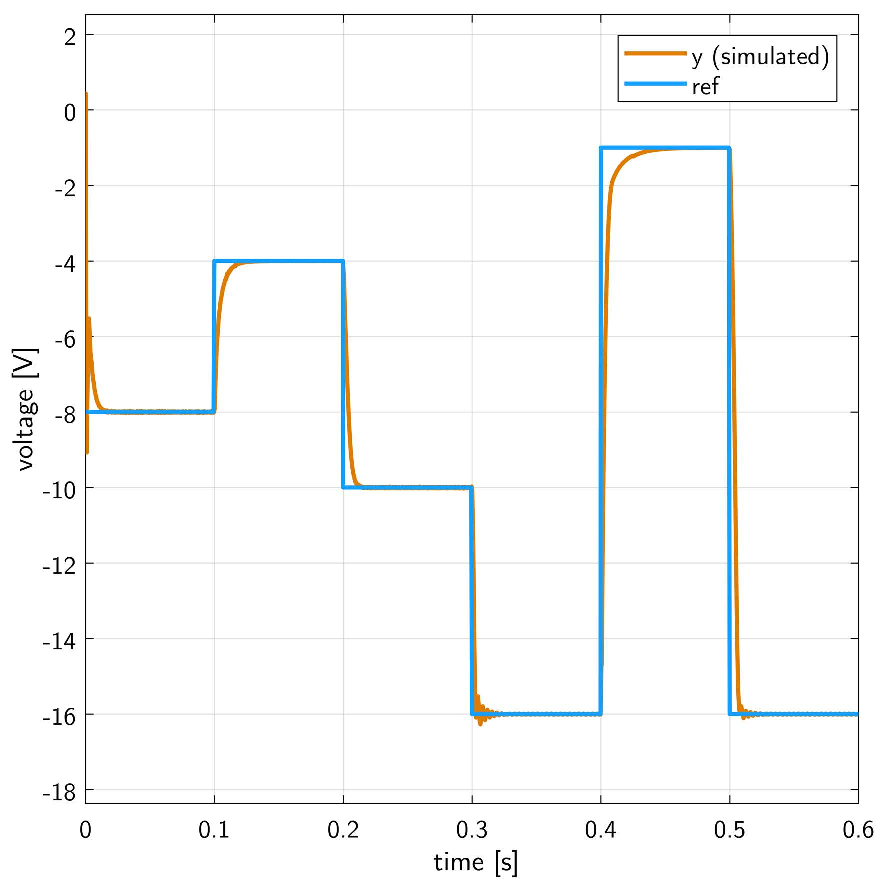
\includegraphics[height = 6cm]{figures/estimation/ref_y_pulsetrain.pdf}
    \caption{Reference train and output voltage response}
    \label{fig:estimatingconditions1}
    \end{subfigure}
    \\[11pt]
    \begin{subfigure}[b]{0.45\textwidth}
    \centering
    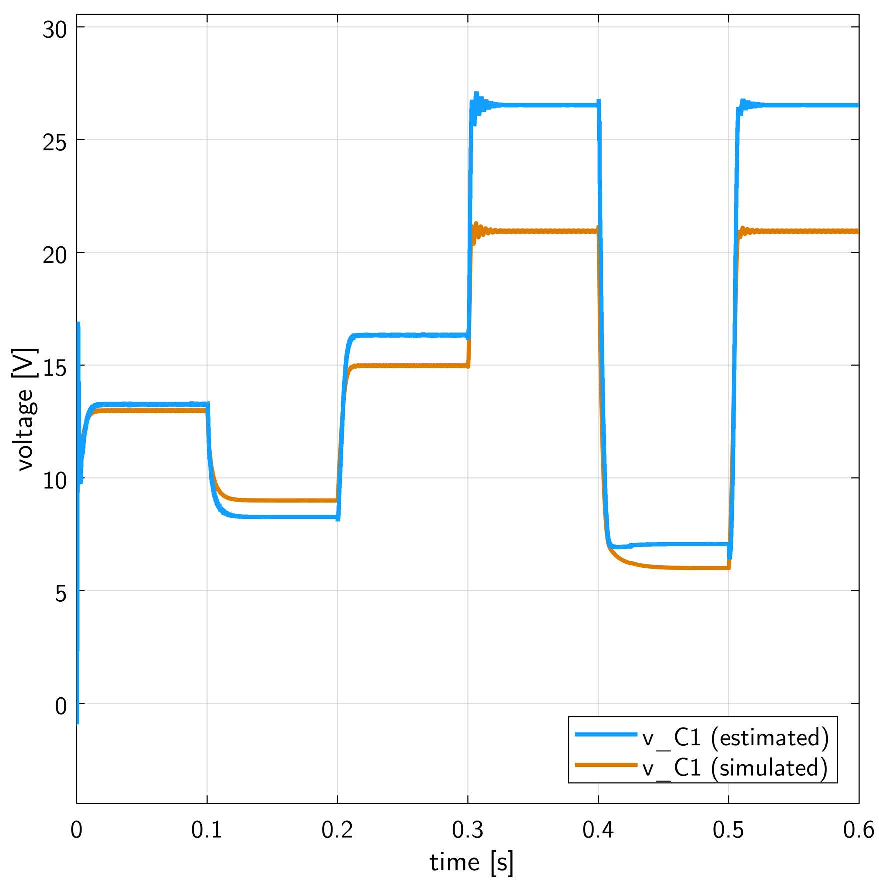
\includegraphics[height = 6cm]{figures/estimation/vC1_vC1.pdf}
    \caption{$v_{C1}$}
    \label{fig:estimatingfirst}
    \end{subfigure}
    \hfill
    \begin{subfigure}[b]{0.45\textwidth}
    \centering
    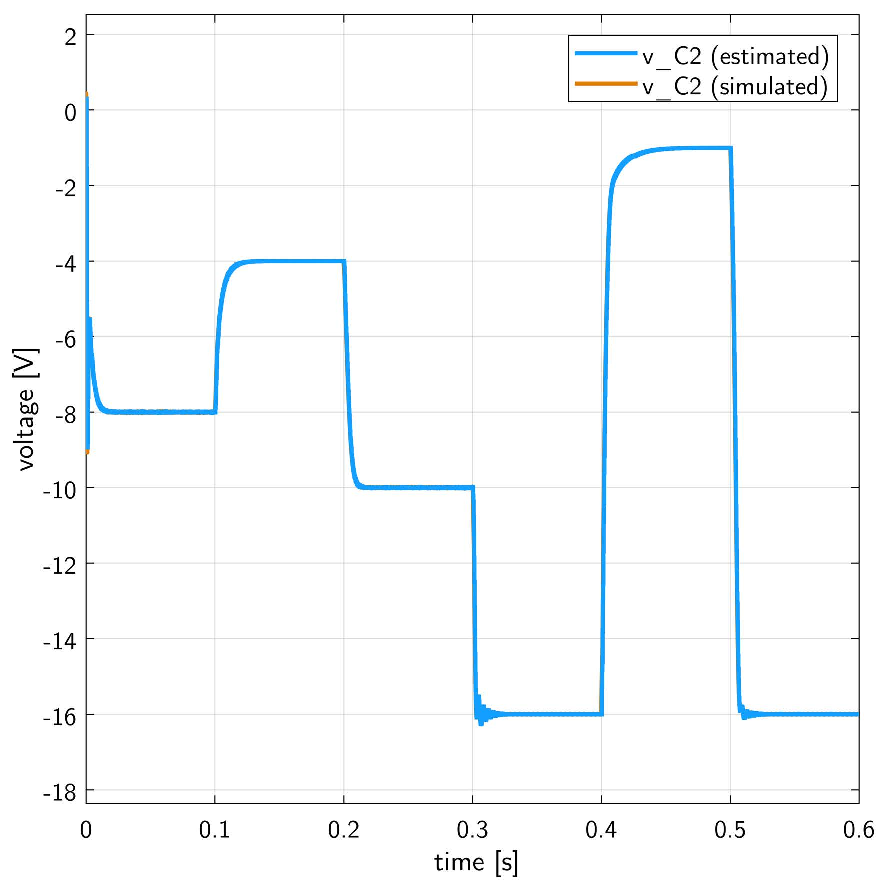
\includegraphics[height = 6cm]{figures/estimation/vC2_vC2.pdf}
    \caption{$v_{C2}$; plots coincide exactly at this scale}
    % \label{}
    \end{subfigure}
    \\[11pt]
    \begin{subfigure}[b]{0.45\textwidth}
    \centering
    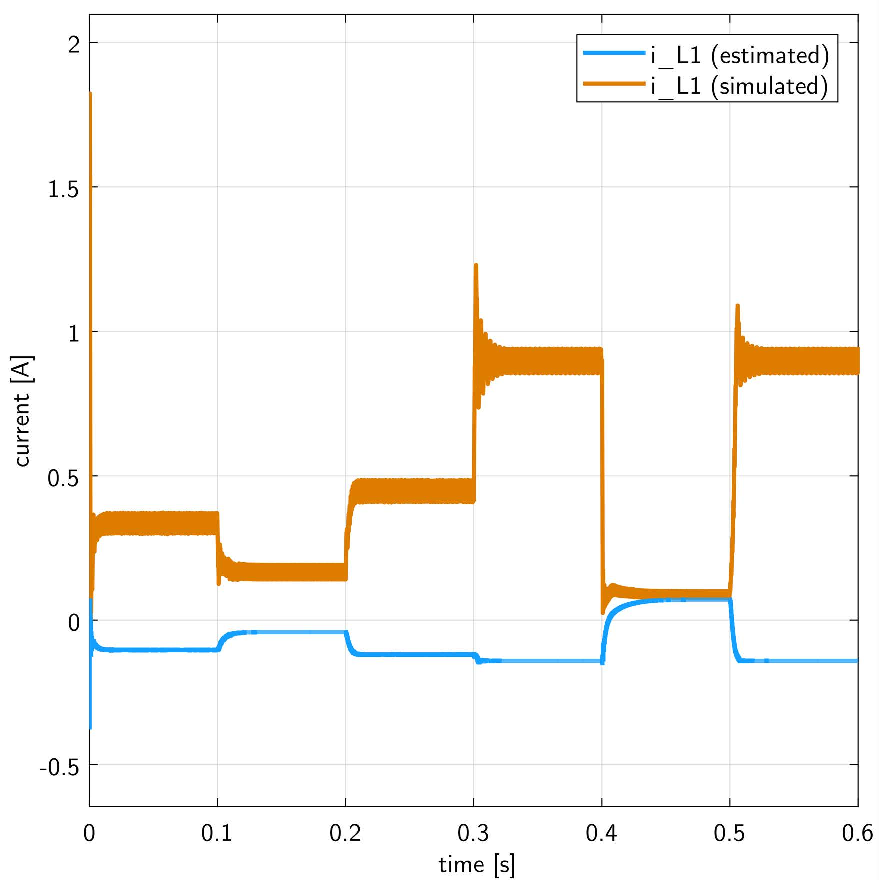
\includegraphics[height = 6cm]{figures/estimation/iL1_iL1.pdf}
    \caption{$i_{L1}$}
    % \label{}
    \end{subfigure}
    \hfill
    \begin{subfigure}[b]{0.45\textwidth}
    \centering
    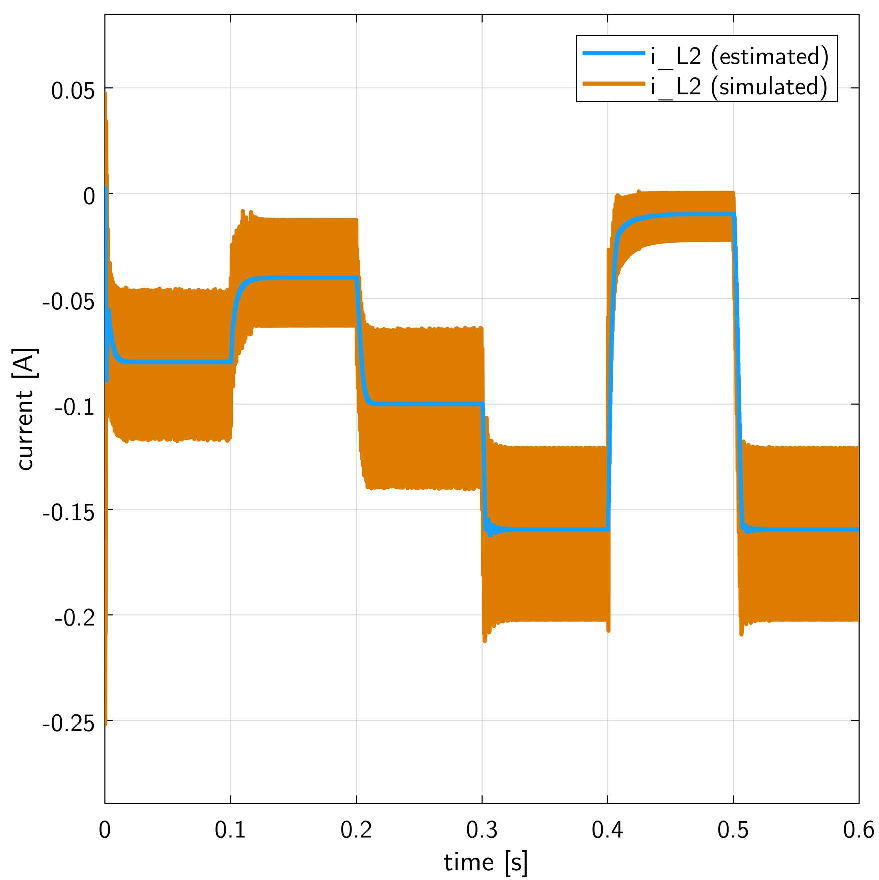
\includegraphics[height = 6cm]{figures/estimation/iL2_iL2.pdf}
    \caption{$i_{L2}$}
    \label{fig:estimatinglast}
    \end{subfigure}
    \end{framed}
    \vspace*{-8mm}
    \caption{Reference train of Figure~\ref{fig:estimatingconditions1} used in generating data of Figures~\ref{fig:estimatingfirst} through~\ref{fig:estimatinglast}}
    \label{fig:estimating}
\end{figure}
%%%%%%%%%%%%%%%%%%%%%%%%%%%%%%%%%%%%%%%%%%%%%%%%%%%%%%%%%%%%%%%%%%%%%%%%%%%%%%%%
\begin{figure}[H]
    \begin{framed}
    \captionsetup[subfigure]{justification = centering}
    \centering
    \begin{subfigure}[b]{0.8\textwidth}
    \centering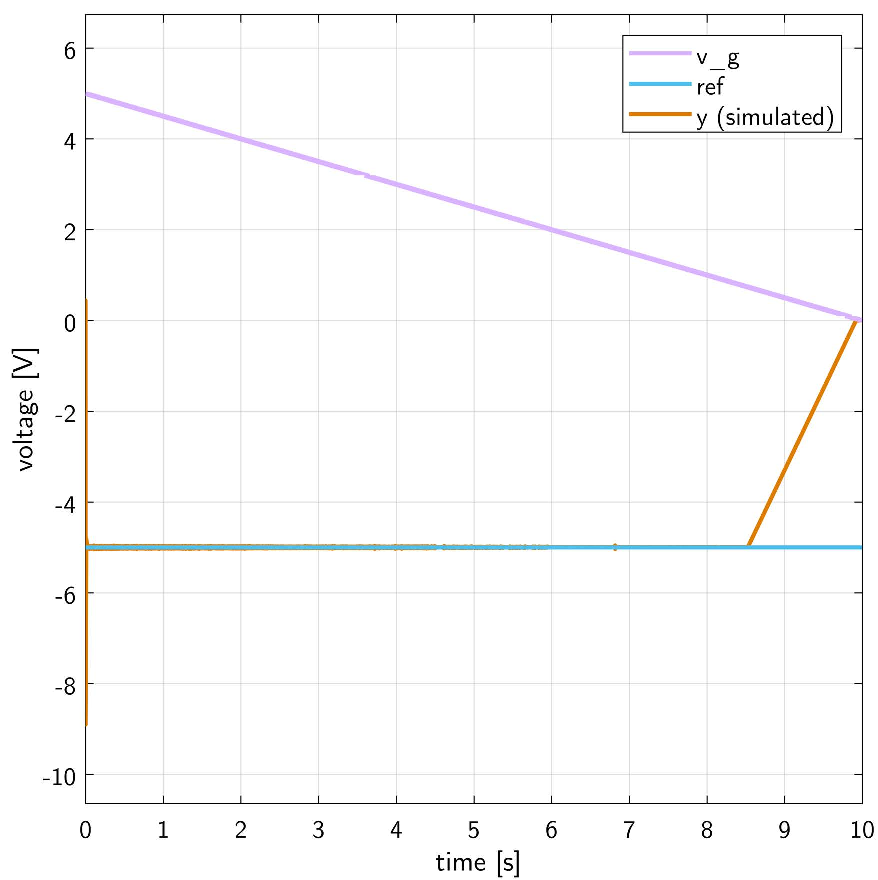
\includegraphics[height = 6cm]{figures/estimation/ref_y_ramp.pdf}
    \caption{Reference voltage, input voltage, and output voltage}
    \label{fig:estimatingconditions2}
    \end{subfigure}
    \\[11pt]
    \begin{subfigure}[b]{0.45\textwidth}
    \centering
    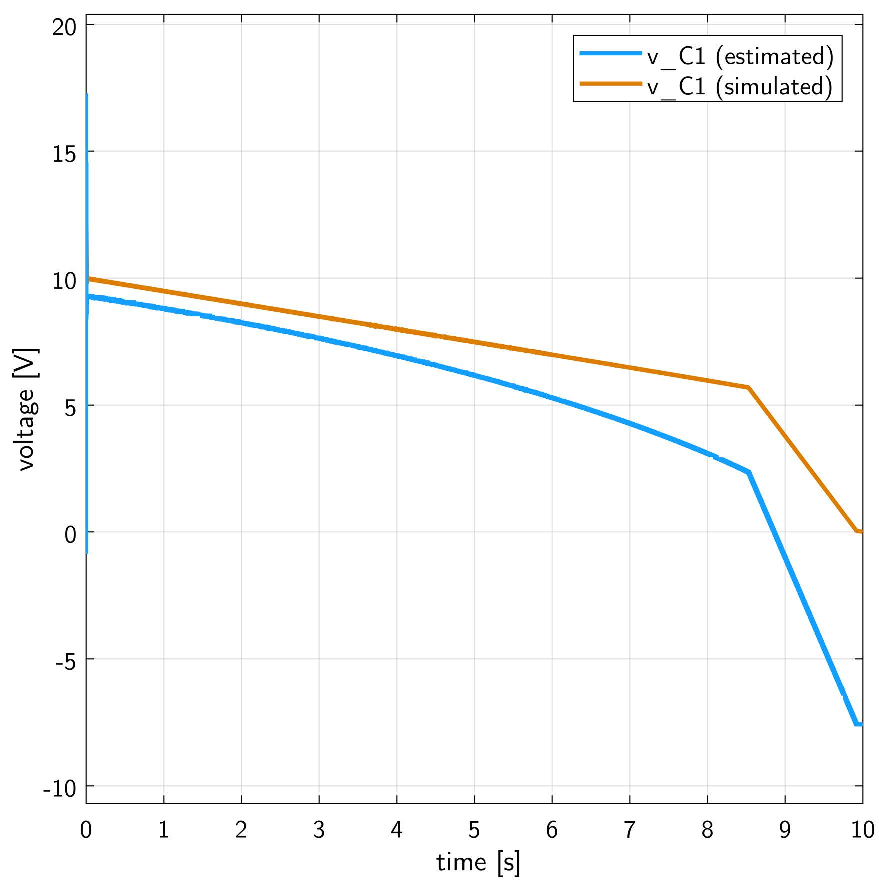
\includegraphics[height = 6cm]{figures/estimation/vC1_vC1b.pdf}
    \caption{$v_{C1}$}
    \label{fig:estimating2first}
    \end{subfigure}
    \hfill
    \begin{subfigure}[b]{0.45\textwidth}
    \centering
    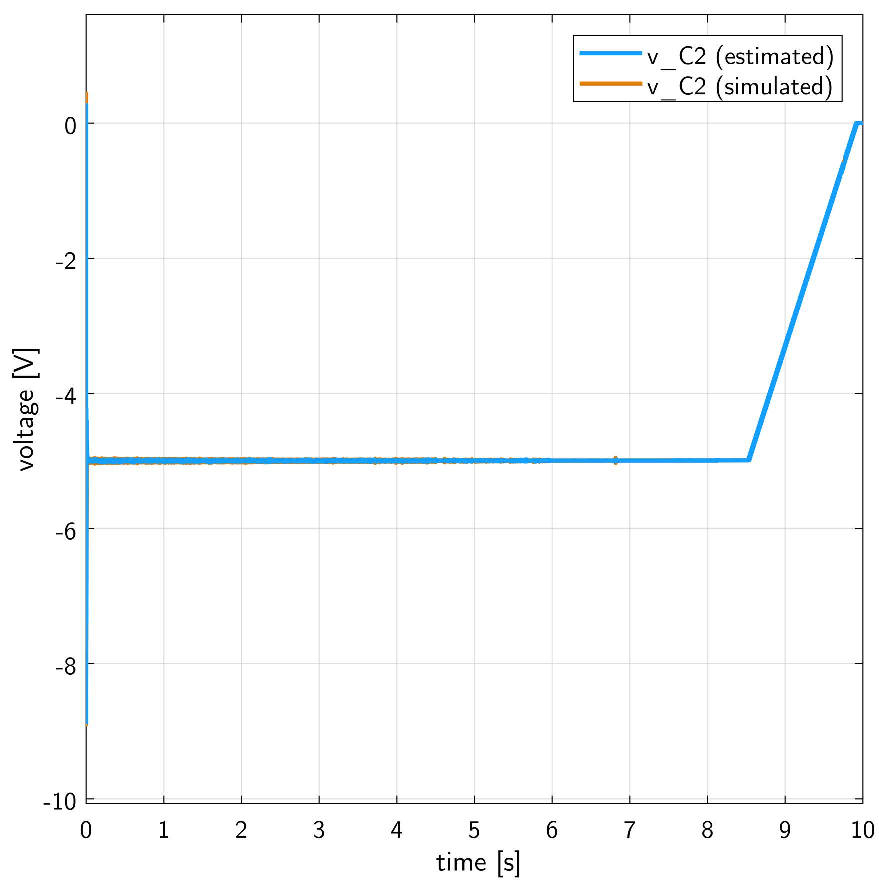
\includegraphics[height = 6cm]{figures/estimation/vC2_vC2b.pdf}
    \caption{$v_{C2}$; plots coincide exactly at this scale}
    % \label{}
    \end{subfigure}
    \\[11pt]
    \begin{subfigure}[b]{0.45\textwidth}
    \centering
    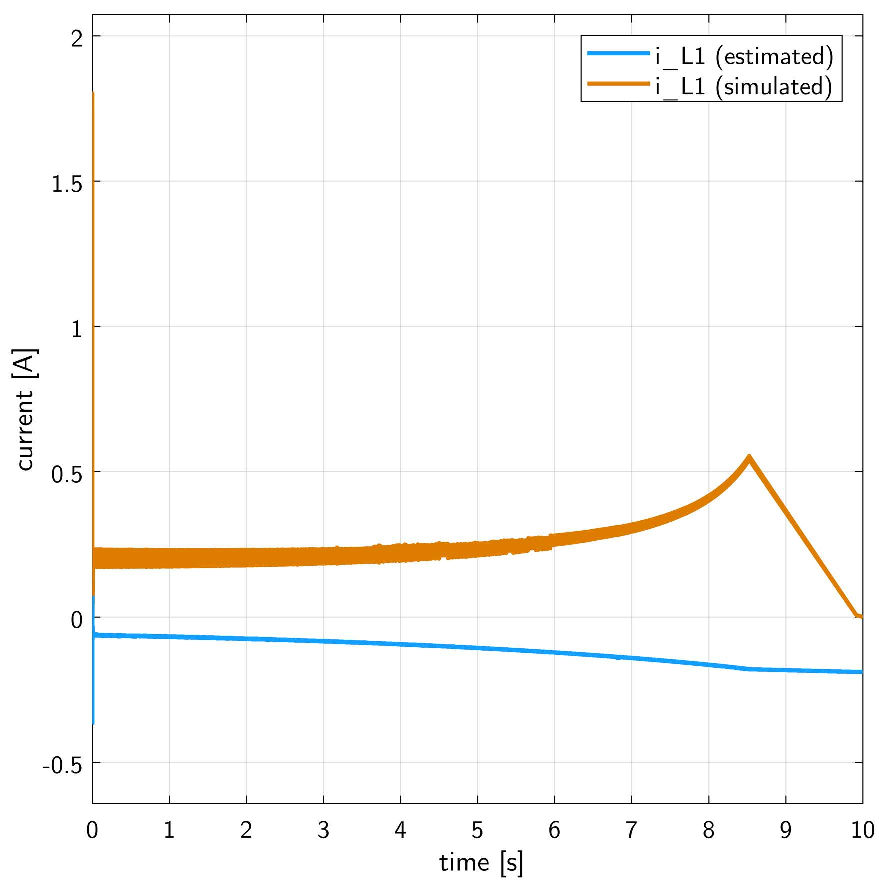
\includegraphics[height = 6cm]{figures/estimation/iL1_iL1b.pdf}
    \caption{$i_{L1}$}
    % \label{}
    \end{subfigure}
    \hfill
    \begin{subfigure}[b]{0.45\textwidth}
    \centering
    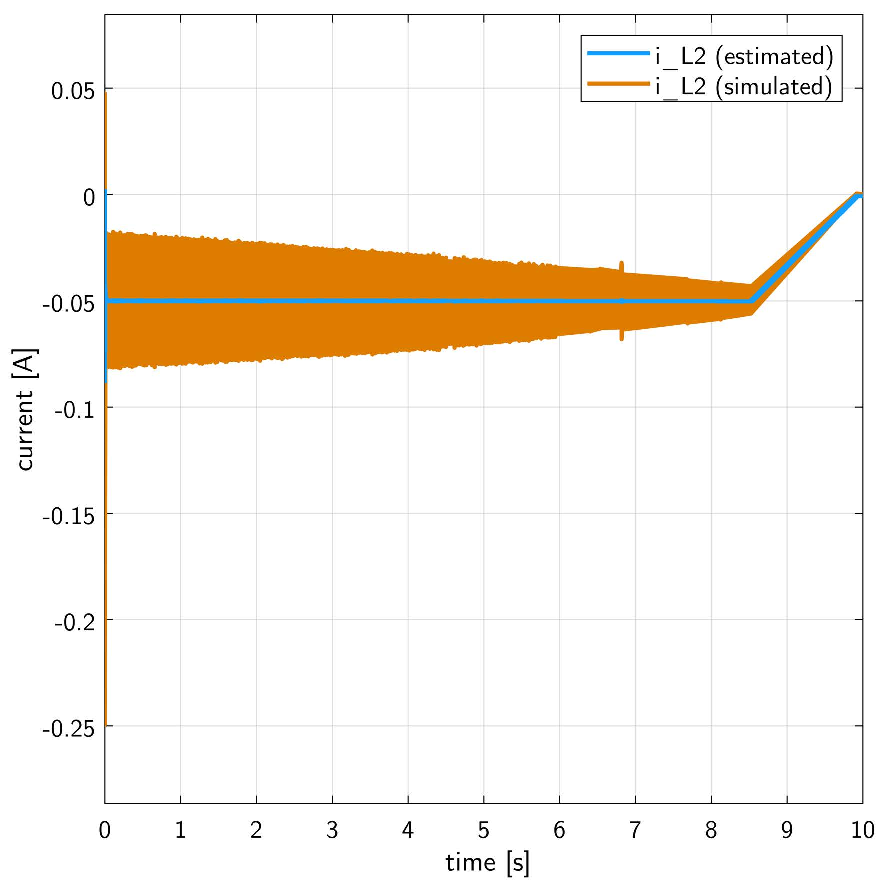
\includegraphics[height = 6cm]{figures/estimation/iL2_iL2b.pdf}
    \caption{$i_{L2}$}
    \label{fig:estimating2last}
    \end{subfigure}
    \end{framed}
    \vspace*{-8mm}
    \caption{Reference and input voltages of Figure~\ref{fig:estimatingconditions2} used in generating data of Figures~\ref{fig:estimating2first} through~\ref{fig:estimating2last}}
    \label{fig:estimating2}
\end{figure}
%%%%%%%%%%%%%%%%%%%%%%%%%%%%%%%%%%%%%%%%%%%%%%%%%%%%%%%%%%%%%%%%%%%%%%%%%%%%%%%%
The response to poor performance of the observer regime was to disable observer state feedback (achieved by setting the LQR weights for system states ($v_{C1}$, $v_{C2}$, $i_{L1}$, and $i_{L2}$) to 0; weight affecting $x_i$ is the only non-zero entry in weight matrix).
%%%%%%%%%%%%%%%%%%%%%%%%%%%%%%%%%%%%%%%%%%%%%%%%%%%%%%%%%%%%%%%%%%%%%%%%%%%%%%%%
%%%%%%%%%%%%%%%%%%%%%%%%%%%%%%%%%%%%%%%%%%%%%%%%%%%%%%%%%%%%%%%%%%%%%%%%%%%%%%%%
\subsection{Hardware}
\subsection{Microcontroller breakout}

\subsection{Controller and ultra-capacitor charging}

\subsection{\'Cuk converter and driving}

%%%%%%%%%%%%%%%%%%%%%%%%%%%%%%%%%%%%%%%%%%%%%%%%%%%%%%%%%%%%%%%%%%%%%%%%%%%%%%%%
%%%%%%%%%%%%%%%%%%%%%%%%%%%%%%%%%%%%%%%%%%%%%%%%%%%%%%%%%%%%%%%%%%%%%%%%%%%%%%%%
\subsection{Programming}
For our controller regime, it is critical that the updated signal be computed before the next ISR being triggered. Reducing the number of instructions results in faster execution time. But also the execution time can be reduced depending on data types used and structure of the code. Extensive code optimisation was undertaken to get the MCU running at the required speed. 

\subsubsection{Exploring different data type}



\textbf{Double}\\
Initially the controller only included integral action and state observer. All the variables were declared as double, as oppose to float. This is because type double is represented with 64 bits providing double the precision. The MCU has 64 kilo bytes memory, which is plentiful for storing all the matrices in double data type. 
Matrix operations were done by computing each element of result matrix. The control loop was run in main infinitely and the frequency was measure by toggling LEDs. It was measured to be roughly 4 kHz. \\

\textbf{Fractional data type}\\
It was then discovered that Microship has own library for digital processors. This library includes matrix operations, such as \texttt{MatrixMultiply}. Most of functions uses fractional arithmetic. Fractional data type is defined as:\\
\texttt{\#ifndef fractional}\\
    \texttt{typedef int fractional;}\\
\texttt{\#endif}

It is represented with 1 sign and 15 fractional bits, ranging between -1 and ($1-2^{-15}$). Any variables declared as double or float can be converte dto fractional type using \texttt{Float2Fract} and vice versa, using \texttt{Fratc2Float}. 

Those functions were tested. When DSP functions were called, the variables were converted to fractional then converted back to float. The frequency was measured in the same and was 2.5kHz. 

After some investigation, it was found that the conversion between the data type is a very expensive operation, especially \texttt{Float2Fract} as it involves division. These two functions were then further investigated. Its execution time was tested by toggling LEDs and the results can be found in Table \ref{tab:conversion}. Note that Number of cycles to toggle LED is not taken into account. 

\begin{table}[h]
\centering
\begin{tabular}{|p{4cm} | c | c|}
\hline
Function    & Frequency & Numer of cycles\\ \hline \hline
Toggling    & 7.5MHz    & 8\\ \hline
Fract2Float & 51kHz     & 1175\\ \hline
Float2Fract & 17.8kHz   & 3370\\ \hline
\end{tabular}
\caption{Convertion time}
\label{tab:conversion}
\end{table}

This demonstrated that the conversion must be avoided as much as possible. Since the matrices for observer are constant, they do not need to be converted every time, it should be converted once at the beginning. Also output form of ADC can be set to either integer or fractional. It was changed to fractional. This removed most of conversion in a loop. This code was tested in the same way and frequency was 4.2kHz. After some testing it was discovered that one of subtraction in fractional data type was taking 100us to compute.

Code was rewritten to avoid the subtraction. It now requires more conversion in a loop, however the frequency was improved to roughly 6.5kHz.\\

These functions were then further investigated. In the source file, it was discovered that the scaling factors of $2^{15}$ and $2^{-15}$ are computed. By defining these constant, this extra computation can be eliminated. So, own conversion functions were written, \texttt{myFratc2Float} and \texttt{myFloat2Fract}. The computational time of these functions was tested in the same way and the result can be found in Table \ref{tab:conversion2}.

\begin{table}[h]
\centering
\begin{tabular}{|p{4cm} | c | p{4cm} | c |}
\hline
Function    & Frequency & Function       & Frequency \\ \hline \hline
Fract2Float & 51kHz     & myFract2Float  & 82.7kHz\\ \hline
Float2Fract & 17.8kHz   & myFloat2Fract  & 24.3kHz\\ \hline
\end{tabular}
\caption{Convertion time comparison}
\label{tab:conversion2}
\end{table}

Slight improvement can be seen and the same control loop with updated conversion functions runs at 7kHz.

Implementing state feedback regime replaces four of \texttt{Fratc2Float} with one matrix multiplication and improves controller performance. It now runs at 6.7kHz. A loop is slower to execute however state feedback regime was included in the final design for better performance. 

%%%%%%%%%%%%%%%%%%%%%%%%%%%%%%%%%%%%%%%%%%%%%%%%%%%%%%%%%%%%%%%%%%%%%%%%%%%%%%%%%%%%%%%%%%%%%%%%%%%%%%%%
%%%%%%%%%%%%%%%%%%%%%%%%%%%%%%%%%%%%%%%%%%%%%%%%%%%%%%%%%%%%%%%%%%%%%%%%%%%%%%%%%%%%%%%%%%%%%%%%%%%%%%%%

\subsubsection{XC16 compilier optimization}
Code optimization was begun by exploring function call. When a function is called, function stack grows. The longer the stack gets, the longer to finish running a code. Function call overhead was tested. First method is LED toggled in main and second is the same but calls a function. The result is provided in Table \ref{tab:stack}. As expected, calling a function required extra time (12 cycles). This suggests that the number of function calls should be minimised. 

\begin{table}[h]
\centering
\begin{tabular}{|p{4cm} | c | c|}
\hline
Function        & Frequency & Numer of cycles\\ \hline \hline
Main            & 7.5MHz    & 8\\ \hline
Function call   & 3kHz      & 20\\ \hline
\end{tabular}
\caption{Function call time}
\label{tab:stack}
\end{table}

Later it was found out that compiler has built in optimisation, which we can enable and select level of optimization between 0 and 3. With full optimization, compiler automatically changes the functions to \texttt{inline} function. Inline function makes the execution faster because it eliminates the function call overheads. Fast floating point math operation was also enabled. The controller on its own now is able to run at 10kHz. However, control loop must be able to run faster than 10kHz to meet the system requirement as ISR and UART communication take time. Further oprimization is required.
%%%%%%%%%%%%%%%%%%%%%%%%%%%%%%%%%%%%%%%%%%%%%%%%%%%%%%%%%%%%%%%%%%%%%%%%%%%%%%%%
%%%%%%%%%%%%%%%%%%%%%%%%%%%%%%%%%%%%%%%%%%%%%%%%%%%%%%%%%%%%%%%%%%%%%%%%%%%%%%%%
% \subsection{Results}
%%%%%%%%%%%%%%%%%%%%%%%%%%%%%%%%%%%%%%%%%%%%%%%%%%%%%%%%%%%%%%%%%%%%%%%%%%%%%%%%
%%%%%%%%%%%%%%%%%%%%%%%%%%%%%%%%%%%%%%%%%%%%%%%%%%%%%%%%%%%%%%%%%%%%%%%%%%%%%%%%
%%%%%%%%%%%%%%%%%%%%%%%%%%%%%%%%%%%%%%%%%%%%%%%%%%%%%%%%%%%%%%%%%%%%%%%%%%%%%%%%